\documentclass[a4paper]{article}
\usepackage[margin=20mm]{geometry}
\usepackage[utf8]{inputenc}
\usepackage{graphicx}
\usepackage[hyphens]{url}
\usepackage{hyperref}
\usepackage{listings}
\usepackage{palatino}

\lstset{frame=tb,
  breaklines=true,
  breakatwhitespace=true,
  columns=flexible,
  gobble=10
}

\title{
  Backy \\
  \Large Simple backup tool \\
  \large Program's characteristics and development directives \\
  \normalsize Version 1.0
}

\author{Marek Felsoci}
\date{\today}

\begin{document}
  \maketitle
  \tableofcontents
  \section{Introduction}
    This document describes backup creation program entitled Backy we are about to develop. Firstly, we are going to decribe program's characteristics such as its purpose and usage. Then we'll define several development directives including programming environment, choosen data structures and program's behavior. Finally, we'll detail program's command line and graphic user interfaces.
  \section{Characteristics}
    \subsection{General purpose}
      It shall be possible thanks to Backy to create a completely new backup of selected drive's or folder's contents but also to maintain an existing backup by being able to reguralry synchronize the backup's contents with those in the source location without having to perform clear backup everytime the source contents change.
    \subsection{Usage description}
      \subsubsection{Backup configuration}
        Once Backy is launched the user have to browse for and choose source contents location. A brief analysis of the source file system will be performed in order to determine the number and the total size of entries to process. \\
        \indent After the preliminary analysis the user have to browse for and choose backup destination location. If the latter already contents any files or folders the user will be prompted whether (s)he wants to reuse these to synchronize the source with or to overwrite existing files or folder with a fresh backup. \\
      \subsubsection{Backup process}
        At this stage Backy is ready to start the backup process. During the backup the program will determine whether the file or folder being processed needs to be copied, ignored or deleted. The program shall display current progress at any moment during the backup. Also it shall be possible to interrupt the backup progress at any time. \\
      \subsubsection{Localization}
        The user interfaces shall be continuously localized to as many languages as possible but initially to US English, French, Slovak, Czech and Ukrainian. All user translation contributions will be greately appreciated. Further information on how to contribute to Backy's localization shall be available in program's GitHub\textsuperscript{\textregistered} repository as well as on the program dedicated website yet to be created.
      \subsubsection{Extension}
        For experienced users it shall be possible to limit the amount of random access memory used by the program for its execution.
  \section{Development directives}
    \subsection{Programming language and environment}
      The program will be developed using C++ language and the open source version of Qt\textsuperscript{\textregistered} Framework will ne used for graphical user interface creation and connection with the program's core. \\
      \indent Initially we intend to develop Linux\textsuperscript{\textregistered} specific version using POSIX functions. The development of a Windows\textsuperscript{\textregistered} specific version using WinAPI is in our plan as well.
    \subsection{Data structure}
      As Backy is supposed to be capable of processing even a large amounts of files and/or folders during backup process we chose a data structure allowing continuous memory usage in order to not to overload random access memory usage and to make possible for experieced users to take control over how much of system memory is being used by Backy. \\
      \indent Core program will use a queue style shared buffer to store useful information related to files and/or folders entries to be backed up. The data structure of a buffer entry is the following:
      \begin{itemize}
        \item \textbf{type} : file or directory (folder)
        \item \textbf{entry path} relatively to source folder or drive
        \item \textbf{size (in bytes)} : only if it's a file
        \item \textbf{date of last modification}
      \end{itemize}
    \subsection{Program's behavior}
      The program will use one producer and one consumer thread in addition to the main thread.
      \subsubsection{Producer thread}
        The producer thread is the simplier one. It will progressively read the source files and/or folders tree from the backup root directory to the furthest leaf and push read entries into the buffer if it's not full. The thread is passively waiting for consumer to consume the entries whenever the buffer becomes full.
      \subsubsection{Consumer thread}
        The most time and disk demanding file operations will be performed by the consumer thread which will progressively process the buffer's entries if there are any. The thread is passively waiting for producer to enqueue new entries whenever the buffer becomes empty and it stops when there is no more entries to process. \\
        \indent On each entry:
        \begin{itemize}
          \item if previous backup exists
            \begin{itemize}
              \item if the entry is a file
                \begin{itemize}
                  \item if the file was already backed up compare the source version with the previously backed up version according to one of the following criteria based on user's initial choice:
                    \begin{itemize}
                      \item date of last modification
                      \item file size
                    \end{itemize}
                    and according to the comparison result then:
                    \begin{itemize}
                      \item overwrite target file
                      \item skip source file
                    \end{itemize}
                  \item if the file was never ever backed up, copy it
                    \begin{itemize}
                      \item copy it
                    \end{itemize}
                  \item if the file no longer exists in the source location then according to user's initial choice (if any)
                    \begin{itemize}
                      \item delete it (default action)
                      \item keep it
                    \end{itemize}
                \end{itemize}
              \item if the entry is a folder
                \begin{itemize}
                  \item if the folder was already backed up
                    \begin{itemize}
                      \item skip it
                    \end{itemize}
                  \item if the folder was never ever backed up
                    \begin{itemize}
                      \item colne it into the backup location (with its full path if it's not a direct descendant of the root folder)
                    \end{itemize}
                  \item if the folder no longer exists in the source location then according to user's initial choice (if any)
                    \begin{itemize}
                      \item delete it recursively (default action)
                      \item keep it with all its content as is
                    \end{itemize}
                \end{itemize}
            \end{itemize}
          \item if there is no previous backup
            \begin{itemize}
              \item if the entry is a file
                \begin{itemize}
                  \item copy it
                \end{itemize}
              \item if the entry is a folder
                \begin{itemize}
                  \item clone it into the backup location (with its full path if it's not a direct descendant of the root folder)
                \end{itemize}
            \end{itemize}
        \end{itemize}
      \subsubsection{Main thread}
        The main thread provides the interaction between the user and the core program whether it's done via command line or graphical user interface. \\
        \indent If either the producer or the consumer encounters an I/O error the user will be prompted to decide whether the program should:
        \begin{itemize}
          \item \textbf{ignore} the entry which caused the error
          \item \textbf{try again}
          \item \textbf{abort} the backup process (no checkpoint is created thus the process will need to start again)
        \end{itemize}
        \indent The main threads also provides a preliminary analysis of the source folder or drive and determines whether the choosen backup destination contains a previous version of backup or not:
        \begin{itemize}
          \item if the target folder or drive is empty do nothing
          \item else prompt the user whether (s)he wants to:
            \begin{itemize}
              \item \textbf{keep} the content and synchronize
              \item \textbf{overwrite} all its content and perform a fresh backup
            \end{itemize}
        \end{itemize}
    \subsection{User interface}
      Backy will be provided with both command line and graphical user interface.
      \subsubsection{Command line}
        The syntax for usage of Backy from command line will be as follows:
        \begin{lstlisting}
          backy <source> <destination> [-s <choice> -c <criterion> -k -m <MBytes> -l <code> -q]
        \end{lstlisting}
        The program's name is immediately followed by paths to the source folder or drive and to the backup destination location.
        Description of Backy's options:
        \begin{itemize}
          \item \textbf{-s} \textit{choice} : if the destination folder or drive is not empty this option will tell the program whether it should keep existing files and use them in backup process to synchronize with source (choice value \textbf{keep} or overwrite all of them and perform a fresh backup (choice value \textbf{overwrite})
          \item \textbf{-c} \textit{criterion} : decides whether the files between source and an existing previous backup are compared by date of last modification (criterion value \textbf{date}) or by size (criterion value \textbf{size})
          \item \textbf{-k} : if an existing previous backup contains files which are no longer present in the source location this option forces the program to keep these files in the backup (the files are deleted if this option is not set)
          \item \textbf{-m} \textit{MBytes} : defines the maximal amount of random access memory in megabytes which should be respected by the program
          \item \textbf{-l} \textit{code} : chooses the language of the program for the current execution
          \item \textbf{-q} : quiet mode (no output excepting errors)
        \end{itemize}
      \subsubsection{GUI}
        The usage of graphical user interface will be far more intuitive.
        \begin{figure}[!ht]
         \centering
         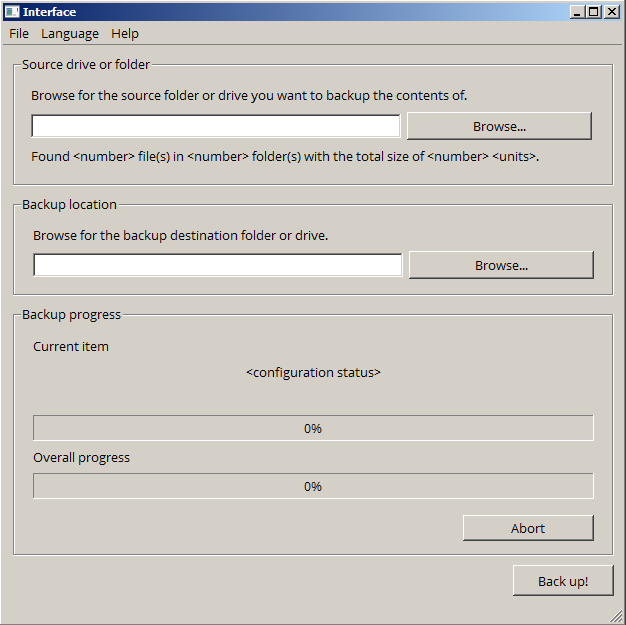
\includegraphics[scale=0.7]{img/interface.png}
         \caption{\textit{Proposed design of Backy's graphical user interface}}
         \label{fig:interface}
        \end{figure}
        \par
        Backy's GUI is divided into multiple sections (groups):
        \begin{itemize}
          \item \textit{Source drive or folder} section allows the user to browse for and choose the source location.
          \item \textit{Backup location} section allows the user to browse for and choose the backup destination location.
          \item \textit{Backup progress} section indicates the backup progress of the current item being processed as well as the overall progress. The \textbf{Abort} button interrupts the backup being performed. If there is no backup in progress then this section is replaced by backup configuration (parameters) summary.
        \end{itemize}
        Main application's menu will allow the user to quit the program, change its language and access online help and information resources. \\
        \indent See figure \ref{fig:interface} for visual details.
  \section{Conclusion}
    Anyone is able to follow the development of Backy and view or obtain its source code by referring to: \url{https://github.com/felsocim/Backy}. \\
    \indent Once released we intend to share Backy for free and license it under the terms of one of open source licenses. All required licensing information will be available in its GitHub\textsuperscript{\textregistered} repository upon the release.
  \section{Legal notices}
    \begin{itemize}
      \item Qt is a registered trademark of The Qt Company Ltd. and its subsidiaries.
      \item Windows\textsuperscript{\textregistered} is a registered trademark of Microsoft Corporation in the United States and/or other countries.
      \item GITHUB\textsuperscript{\textregistered} is exclusive trademark registered in the United States by GitHub, Inc.
      \item Linux\textsuperscript{\textregistered} is the registered trademark of Linus Torvalds in the U.S. and other countries.
      \item OpenSans font used for graphic user interface design is licensed under the terms of Apache License Version 2.0 available at: \url{https://www.apache.org/licenses/LICENSE-2.0}
    \end{itemize}
    All other content of this document is publicly available under the terms of Creative Commons Attribution NonCommercial ShareAlike 4.0 International available at: \url{http://creativecommons.org/licenses/by-nc-sa/4.0/}.
\end{document}
